%!TEX root = TDT4265-Summary.tex
\section{Frequency filtering}

\begin{equation}
    \euler^{\ramuno \theta}
    =
    \cos \theta
    +
    \ramuno \sin \theta
\end{equation}

%%%%%%%%%%%%%%%%%%%%%%%%%%%%%%%%%%%%%%%%%%%%%%%%%%%%%%%%%%%%
\subsection{Fourier transformation}

\subsubsection{1D continuous Fourier transform (CFT)}
The following equations define the forward and backward CFTs:
\begin{gather}
    F(u) = \int_{-\infty}^{\infty} f(x) \euler^{-2 \pi u x} \dif x \\
    f(x) = \int_{-\infty}^{\infty} F(u) \euler^{\ramuno 2 \pi u x} \dif u \\
\end{gather}
In many fields $f(x)$ is a function of time, but in image processing it is usually a function that maps from spatial position in an image to image intensity. Then $F(u)$ is a complex function of frequency, with a magnitude and phase (usually only magnitude is displayed).

\subsubsection{2D discrete Fourier transform (DFT)}
Digital images have discrete values, and are 2D, so we need a 2D DFT to convert them to the frequency domain. For an image of size $M \times N$, it is
\begin{equation}
    F(u,v)
    =
    \sum_{x=0}^{M-1}
    \sum_{y=0}^{N-1}
    f(x,y)
    \euler^{-\ramuno 2 \pi (\frac{ux}{N}+\frac{vy}{N})}
\end{equation}
and the inverse transform is
\begin{equation}
    f(x,y)
    =
    \frac{1}{MN}
    \sum_{u=0}^{M-1}
    \sum_{v=0}^{N-1}
    F(u,v)
    \euler^{\ramuno 2 \pi (\frac{ux}{M}+\frac{vy}{N})}
    .
\end{equation}

\begin{figure}[htbp]
    \hfill
    \subfigure[Intensity image]{
\includegraphics[width=.45\linewidth]{images/sin3.png}}
    \hfill
    \subfigure[Frequency image]{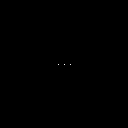
\includegraphics[width=.45\linewidth]{images/sin3real.png}}
    \hfill
    \caption{An image and its Fourier transform}
\end{figure}

%%%%%%%%%%%%%%%%%%%%%%%%%%%%%%%%%%%%%%%%%%%%%%%%%%%%%%%%%%%%
\subsection{Convolution}

\paragraph{Convolution theorem} Convolution in one domain is equal to multiplication in the other:
\begin{equation}\label{eq:convolution-theorem}
\begin{split}
    h(x) \conv f(x) &\iff H(x) \cdot F(x) \\
    h(x) \cdot f(x) &\iff H(x) \conv F(x)
\end{split}
\end{equation}

%%%%%%%%%%%%%%%%%%%%%%%%%%%%%%%%%%%%%%%%%%%%%%%%%%%%%%%%%%%%
\subsection{The sampling theorem}
If samples are taken at a rate over twice the highest frequency of a function, it can be recreated without loss of information. This limit is the sampling theorem:
\begin{equation}
    \frac{1}{\Delta T} > 2 \mu\sub{max}
\end{equation}

%%%%%%%%%%%%%%%%%%%%%%%%%%%%%%%%%%%%%%%%%%%%%%%%%%%%%%%%%%%%
\subsection{Basics of frequency domain filtering}
Filtering of an image $F(u,v)$ in the frequency domain with a filter $H(u,v)$ is done by
\begin{equation}
    g(x,y) = \fourier^{-1}[H(u,v) F(u,v)]
\end{equation}
where $H$ is a matrix of equal size to the image. (The multiplication $H F$ is done elementwise.)

\paragraph{Shifting}
To obtain a centered Fourier transform, multiply the image by $(-1)^{x+y}$ before transforming. Then $F(0,0)$ will be at the center. Alternatively swap the quadrants after transforming.

%%%%%%%%%%%%%%%%%%%%%%%%%%%%%%%%%%%%%%%%%%%%%%%%%%%%%%%%%%%%
\subsection{Frequency domain smoothing}

\subsubsection{Ideal low-pass filter (ILPF)}
An ILPF is a filter with no attenuation for frequencies below a threshold (the \emph{cutoff frequency}), and full attenuation for all frequencies above:
\begin{equation}
    H(u,v) =
    \begin{cases}
        1 \quad\mbox{if } D(u,v) \leq D_0 \\
        0 \quad\mbox{if } D(u,v) >    D_0
    \end{cases}
\end{equation}
The spatial representation of the ILPF is the $\sinc$ function (in 2D, that means any cross-section through the origin is a $\sinc$ function).

The convolution theorem \eqref{eq:convolution-theorem} then reveals why the ringing effect occurs: Multiplying with an ILPF in the frequency domain is equivalent to convolving with a $\sinc$ filter (Figure \ref{fig:sinc}) in the spatial domain.

\begin{figure}[htbp]
    \centering
    % 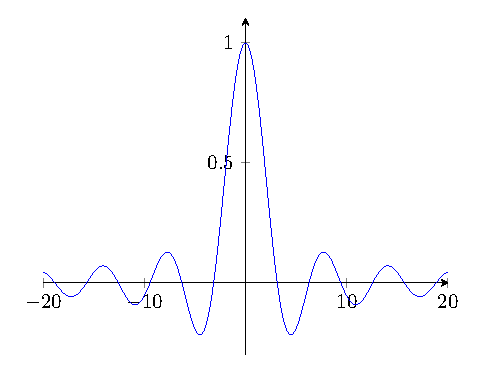
\includegraphics[width=.8\linewidth]{images/sinc_x_plot}
    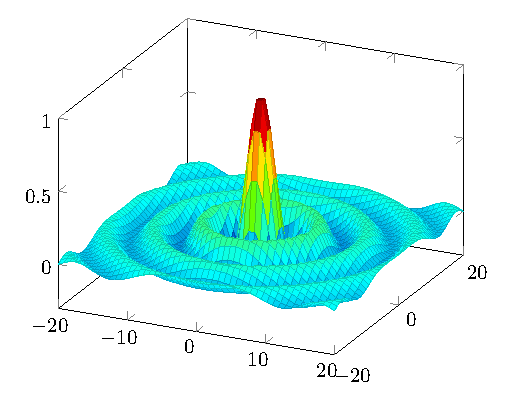
\includegraphics[width=.8\linewidth]{images/sinc_2d_plot}
    \caption{The $\sinc$ function}
    \label{fig:sinc}
\end{figure}

\subsubsection{Butterworth low-pass filter (BLPF)}
Defined as
\begin{equation}
    H(u,v)
    =
    \frac{1}{1 + [D(u,v)/D_0]^{2n}}
\end{equation}
where $n$ is the order and $D(u,v)$ is the distance in the frequency domain between $(u,v)$ and the center. This gives a smooth cutoff, which reduces ringing (depending on order). Order 1 has no ringing, 2 very little, and higher orders may have visible ringing. (A BLPF with $n = \infty$ is equal to an ILPF.)

\subsubsection{Gaussian low-pass filter (GLPF)}
Given in 2D as
\begin{equation}
    H(u,v) = \euler^{-\frac{D^2(u,v)}{2 D_0}}.
\end{equation}

The inverse Fourier of this is also a Gaussian function, so it will have no ringing. It's pretty nice.

\subsubsection{Some examples of lowpass filtering}
\begin{itemize}
    \item Smoothing digitized text to fill gaps and improve legibility, especially for machine processing.
    \item Cosmetic processing, such as softening skin on images of people.
    \item Removing artifacts, such as noise and scan lines.
    \item However, smoothing is mostly used for preprocessing.
\end{itemize}

%%%%%%%%%%%%%%%%%%%%%%%%%%%%%%%%%%%%%%%%%%%%%%%%%%%%%%%%%%%%
\subsection{Frequency domain sharpening}
Done with high-pass filters, which are pretty much the opposite of low-pass filters:
\begin{equation}\label{eq:frequency-hp-lp-relation}
    H\sub{highpass}(u,v) = 1 - H\sub{lowpass}(u,v)
\end{equation}

\subsubsection{Ideal high-pass filter (IHPF)}
Defined as
\begin{equation}
    H(u,v) =
    \begin{cases}
        0 \quad\mbox{if } D(u,v) \leq D_0 \\
        1 \quad\mbox{if } D(u,v) >    D_0
    \end{cases}
\end{equation}

\subsubsection{Butterworth high-pass filter (BHPF)}
\begin{equation}
    H(u,v) =
    \frac{1}{1 + [D_0 / D(u,v)]^{2n}}
\end{equation}

\subsubsection{Gaussian high-pass filter (GHPF)}
\begin{equation}
    H(u,v) = 1 - \euler^{-\frac{D^2(u,v)}{2 D_0^2}}
\end{equation}

\subsubsection{Frequency domain Laplacian filter}
The Laplacian works the same way in the frequency domain as in the spatial domain. With
\begin{equation}
    H(u,v) = -4\pi^2(u^2 + v^2)
\end{equation}
the Laplacian image is
\begin{equation}
    \nabla^2 f(x,y) = \fourier^{-1} \left\{ H(u,v) F(u,v) \right\}
\end{equation}
and the enhanced image is
\begin{equation}
    g(x,y) = f(x,y) + c \nabla^2 f(x,y)
\end{equation}

\subsubsection{Unsharp masking, highboost filtering, high-frequency emphasis filtering}
Like in the spatial domain \eqref{eq:unsharp-masking}, unsharp masking and highboost filtering can be be done in the frequency domain:
\begin{equation}
\begin{split}
    g(x,y)
    &=
    \fourier^{-1}
    \left\{
        \left[
            1 + k \cdot [1 - H\sub{LP}(u,v)]
        \right]
        F(u,v)
    \right\} \\
    &=
    \fourier^{-1}
    \left\{
        [1 + k \cdot H\sub{HP}(u,v)] F(u,v)
    \right\}
\end{split}
\end{equation}
Remember \eqref{eq:frequency-hp-lp-relation}. This leads to the high-frequency emphasis filter
\begin{equation}
    g(x,y)
    =
    \fourier^{-1}
    \left\{
        [k_1 + k_2 \cdot H\sub{HP}(u,v)] F(u,v)
    \right\}
\end{equation}
where $k_1 \geq 0$ is the DC term, and $k_2 \geq 0$ sets the contribution of high frequencies. By setting a nonzero DC term, the low frequency grey levels is not lost. High-frequency emphasis filtering followed by histogram equalization can enhance clarity and detail significantly, and is useful for e.g. X-ray images.

%%%%%%%%%%%%%%%%%%%%%%%%%%%%%%%%%%%%%%%%%%%%%%%%%%%%%%%%%%%%
\subsection{Selective filters}
These filters only affect parts of the frequency spectrum.

\subsubsection{Bandreject and bandpass}
Filters that remove all frequencies inside or outside a given range. Like normal filters, these can be created as ideal, Butterworth, or Gaussian filters.

\subsubsection{Notch filters}
These filters reject (or pass) frequencies at chosen locations in the frequency rectangle. A common example is removing periodic noise, such as moiré.
